% $  Id: collabide.tex  $
% !TEX root = main.tex

%%
\section{CollabIDE}
\label{sec:collab-ide}

CollabIDE\footnote{\url{https://collabide.herokuapp.com/}} is a cloud-based integrated development environment presenting collaboration facilities 
for distributed development teams working on a software project. \fref{fig:general-view} shows the 
general view of a project created with the IDE. 
CollabIDE has three key features which help to reduce the overhead of managing versions or product variants. These features are:
\begin{enumerate*}[label=(\arabic*)] 
\item version management, 
\item product variant management, and 
\item collaborative development.
\end{enumerate*}

\begin{figure}[tbp]
  \centering
  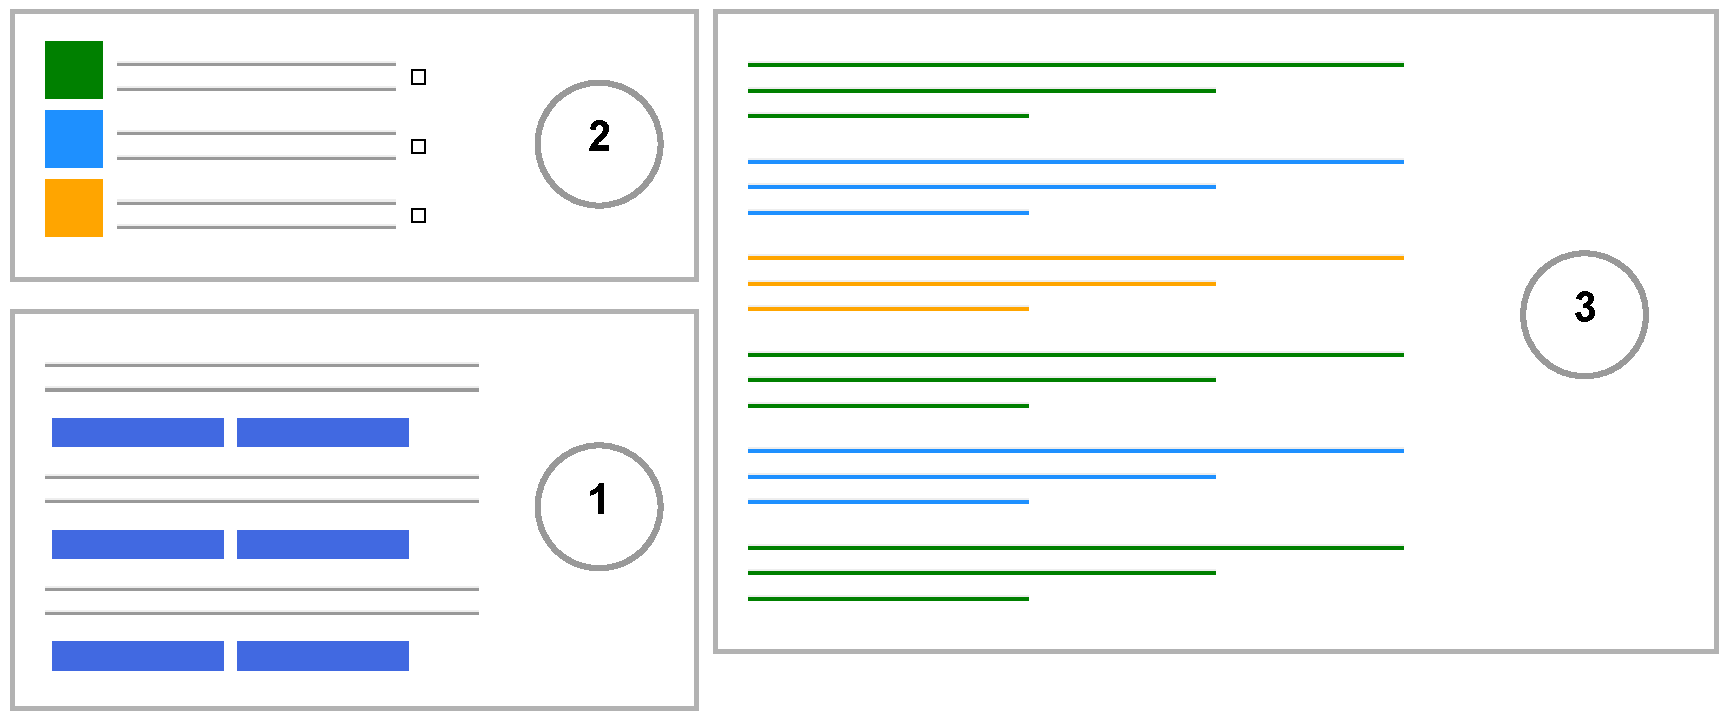
\includegraphics[width=0.7\textwidth]{img/collabIDEGeneral}
  \caption{General view of CollabIDE}
  \label{fig:general-view}
\end{figure}

%%
\subsection{Version Management}
\label{sec:vcs}
Software products evolve over time~\cite{lehman02}. Rather than releasing a fully working product at 
once, developers implement products incrementally. Each product increment focuses on a single 
feature or part of the functionality at a time. Each of these features marks a new \emph{version} of the 
system, moving forward linearly in time. Defining and synchronizing between these pieces of 
functionality must be carried out multiple times in a project's lifespan. In the long-term, this process 
has a lasting impact in the productivity.

CollabIDE takes the association between a feature's development, and program versions to an 
extreme. In CollabIDE, every code modification (regardless of its size) is marked as a new product 
increment. Furthermore, instead of asking developers to continuously create and manage product 
versions, CollabIDE automatically generates versions for each code increment. These increments are 
identified by a set of variables relevant to the project development. For example, relevant information 
to generate versions may include the developer's name, or the time of the day. Additionally, if 
developers want to create their own versions, it is possible to do so simply by giving them a name in 
the versions pane of the interface. \fref{fig:versions} shows the way product versions are 
managed in CollabIDE. 

A differentiating feature of CollabIDE is that versions are live. That is, every time a new version is 
created by any of the developers, it is made available to all developers immediately. 
As a consequence, versioning conflicts become nonexistent since developers see the latest 
version of the code at all times. Moreover, when switching between versions, developers have an 
immediate view of the complete state of the code at the moment the version was created or edited. 

\begin{figure}[tbp]
  \centering
  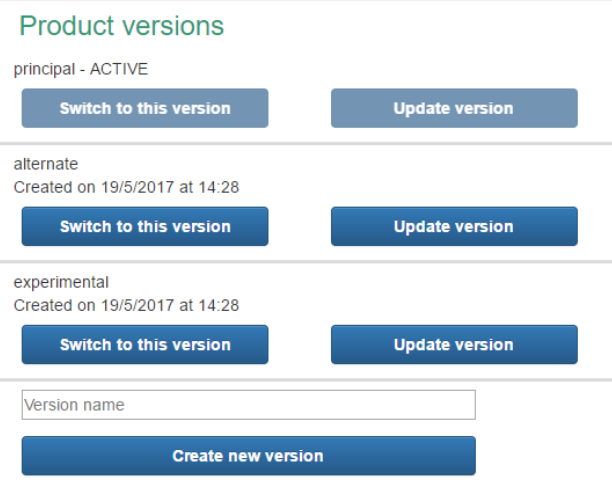
\includegraphics[width=0.45\textwidth]{img/fig4-collabIDEVersionManagement}
  \caption{Version visualization and management in CollabIDE}
  \label{fig:versions}
\end{figure}

The facilities for version management in CollabIDE help reduce the long-term impact of creating, 
updating, and synchronizing product versions, as these processes occur autonomously upon simple 
interactions.

%%
\subsection{Product Variant Management}
\label{sec:product-variant}
In \ac{SPL} development, product variants are managed through variability models, describing the 
different components of the product, and the different options for each of these 
components~\cite{pohl05}. A product variant consists of the composition of a base product with 
different features, usually specialized for each costumer or purpose. This process requires developers 
to define beforehand both, the base product, and the variation points (\ie those features that can be 
interchanged with other features). This process is time consuming for the project setup, and fixed in 
the points where variations may take place.

CollabIDE takes advantage of its \ac{VCS} to enable a more flexible product variation model. Product 
variants are defined by the composition of the different versions available in the system. These 
versions may be chosen based on the time of their creation (as explained in the previous section), or 
taking into account the contributions made by specific developers. The composition takes place 
behind the scene using \ac{COP} facilities for dynamic software composition (\cf 
\fref{sec:implementation}).

\fref{fig:contribution} shows the panel in the CollabIDE interface to select the different variants, in this 
case according to developers' contributions. Selecting one of the contributions renders the associated 
code as part of the interface, and composes the variant with the currently working code. From a 
product variant point of view, this feature eases the process of building new variants from existing 
fragments of code, effectively reducing the overhead derived from executing initial configuration 
processes.

\begin{figure}[htbp]
  \centering
  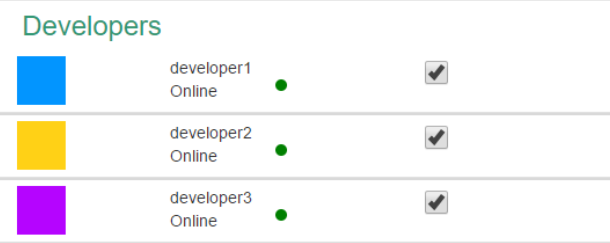
\includegraphics[width=0.45\textwidth]{img/fig3-collabIDEContributionManagement}
  \caption{Product composition through contribution selection}
  \label{fig:contribution}
\end{figure}


%%
\subsection{Collaborative Development}

CollabIDE offers a feature for collaborative development. Taking advantage of the \ac{VCS}, developers 
are able to work concurrently on the same code base, having immediate feedback about the 
contributions of other developers.
Developers' code is differentiated by highlighting, in a unique color, the code contributed by each 
developer, as shown in \fref{fig:layers}. First, colored code, offers a first-hand view about the 
contributions of each team member, increasing awareness  about code owners, and coordination to 
develop or fix code increments. Second, code highlighting is used as a means to identify features a 
developer has worked on, enabling the composition of specific product variants by selecting the work 
of developers associated to specific features. 

\begin{figure}[htbp]
  \centering
  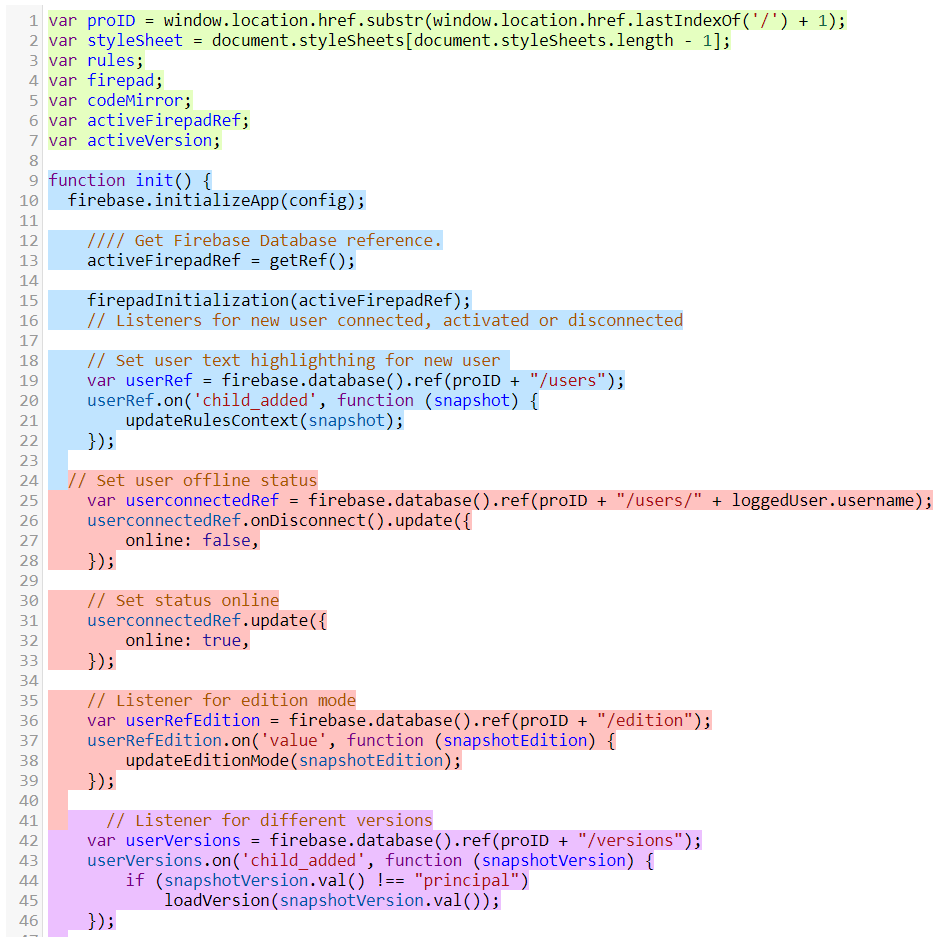
\includegraphics[width=0.7\textwidth]{img/fig2-collabIDEConcurrentProgramming}
  \caption{First-hand view of developers' contributions}
  \label{fig:layers}
\end{figure}


%%
\subsection{Implementation}
\label{sec:implementation}

The implementation of CollabIDE is based on the \acf{COP} paradigm, incorporated in Firepad.\footnote{\url{https://firepad.io/\#1}}

%%%%
\subsubsection{\ac{COP} in a Nutshell}
\ac{COP} is a programming paradigm designed for the dynamic adaptation of software systems based 
on context information gathered from the system's surrounding execution 
environment~\cite{salvaneschi+12survey}. \ac{COP} consists of three main abstractions: 
\emph{Contexts}, \emph{Behavioral adaptations}, and \emph{Context activations}.

\paragraph{Contexts} represent semantically meaningful situations gathered from a system's 
surrounding environment~\cite{dey01}. Contexts are defined as first-class entities of the system that 
are manipulated in reaction to external stimulus (\eg changes in sensed information, actions executed 
by users). A context can be in an active state, stating that the situation it represents is taking place in 
the surrounding environment. Otherwise, the context is said to be inactive.

\paragraph{Behavioral adaptations} are fine-grained behavior definitions associated to one or several 
context entities. Behavioral adaptations dictate the observable behavior of a system under a particular 
situation sensed from the surrounding environment. The combination of behavioral adaptations and 
contexts constitute what we call an \emph{adaptation}.

\paragraph{Context activations} correspond to the systems' reaction to the surrounding environment. 
Whenever a context is sensed to be active (the information associated with the contexts satisfies a 
given activation condition), an activation message is sent to the system. Upon the message's 
evaluation, the system is dynamically recomposed taking into account all behavioral adaptations 
associated with the context. This process may overwrite previous behavior definitions already 
composed in the system. Whenever the activation conditions of a context are unsatisfied, a 
deactivation message is sent, effectively withdrawing the behavioral adaptations associated with the 
context. That is, the system is dynamically recomposed, not taking into account the context's 
behavioral adaptations.  Note that, different combinations of contexts may compose the system at a 
time.


%%%%
\subsubsection{CollabIDE Internals}
To implement the features described in \fref{sec:collab-ide}, we create a one to one association 
between adaptations and versions.
Versions consist of the code introduced by developers and the conditions of the surrounding 
environment in which these take place. 

As a cloud-based platform, CollabIDE is implemented in ECMAScript, using 
node.js\footnote{\url{http://nodejs.org/}} for the backend, and 
Firepad, an open source collaborative text editor, for the frontend.
To define and manage contexts we use Context Traits~\cite{gonzalez13}. 

As mentioned before, versions and product variants are defined based on the time in which a code 
increment is defined, and the user defining such increment, respectively. Each of these situations 
defines a condition in which the code is created; therefore, they constitute contexts.
First, whenever users log into the system, a context is automatically defined
using the timestamp as its identifier. The following snippet show the example of a context created 
for a contribution made on 19/05/2017 at 14:28
\vspace{-4ex}
\begin{ctxtraits}
 var 190520171428 = new cop.Context{
   name: "190520171428"
 }
\end{ctxtraits}
\vspace{-4ex}

Additionally, the system defines a context per user, associating all code increments to this context too. 
The purpose of this additional association is twofold. On the one hand, we use it to select product 
variants per user. On the other hand, it is used to adapt the behavior of the text rendering in Firebase, 
in order to display the colored layer indicating the contributions for each developer.

All code increments are recorded as part of a behavioral adaptation associated to a context. The 
following code snippet defines the behavioral adaptation (Lines \ref{ln:ba-init}-\ref{ln:ba-end}) to modify 
the text highlighting feature for a particular developer. Behavioral adaptations are then
associated to contexts (\fref{ln:association}) to be used in the system, in this case adapting the 
\scode{defineVisibility} function of the \scode{highlighter} Firebase object. In this example, as a 
particular developer is selected (as in \fref{fig:contribution}), this activates the \ctx{DevContext}, 
coloring the text with the color associated to the developer. The \scode{proceed} call in \fref{ln:proceed} 
works as a super-call, to invoke the original behavior of the system (\ie without adaptation)

\vspace{-3.5ex}
\begin{ctxtraits}[numbers=left]
 HighlightTrait = Trait = ({ ` \label{ln:ba-init} `
   defineVisibility : function() {
     developerRule.style.display = "inline";
     this.proceed();  `\label{ln:proceed} `
   }
 })` \label{ln:ba-end} `
 DevContext.adapt(highlighter, HighlightTrait); ` \label{ln:association} `
\end{ctxtraits}
\vspace{-4ex}

\endinput
